\chapter{Specific requirements}

\section{External interface requirements}

The system provides all the main functions described in section 2.2.1.
Users are able to access all the information they are granted permission for.
Given such purposes, any device is suitable to make use of all the S\&C functionalities, allowing convenient acces through any web browser.

\subsection{User Interfaces}

\begin{figure}[H]
    \centering
    \begin{minipage}{0.45\textwidth}
        \centering
        \fcolorbox{gray}{white}{
            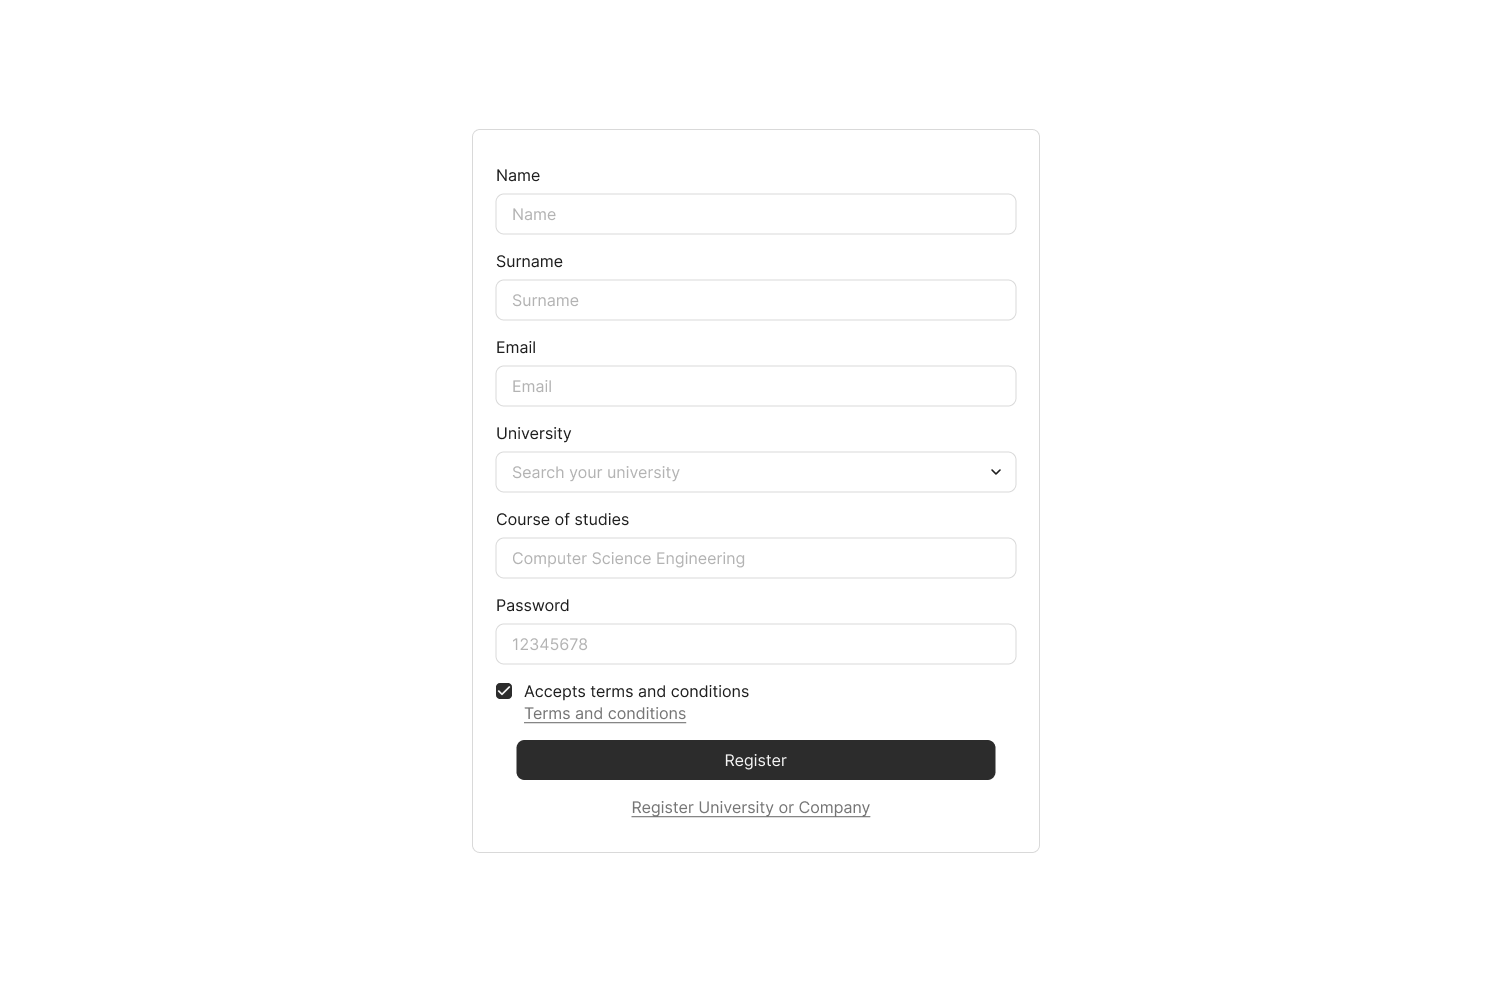
\includegraphics[width=\linewidth]{../../assets/user-interfaces/signup.png}
        }
        \subcaption{Sign up page}
    \end{minipage}
    \hfill
    \begin{minipage}{0.45\textwidth}
        \centering
        \fcolorbox{gray}{white}{
            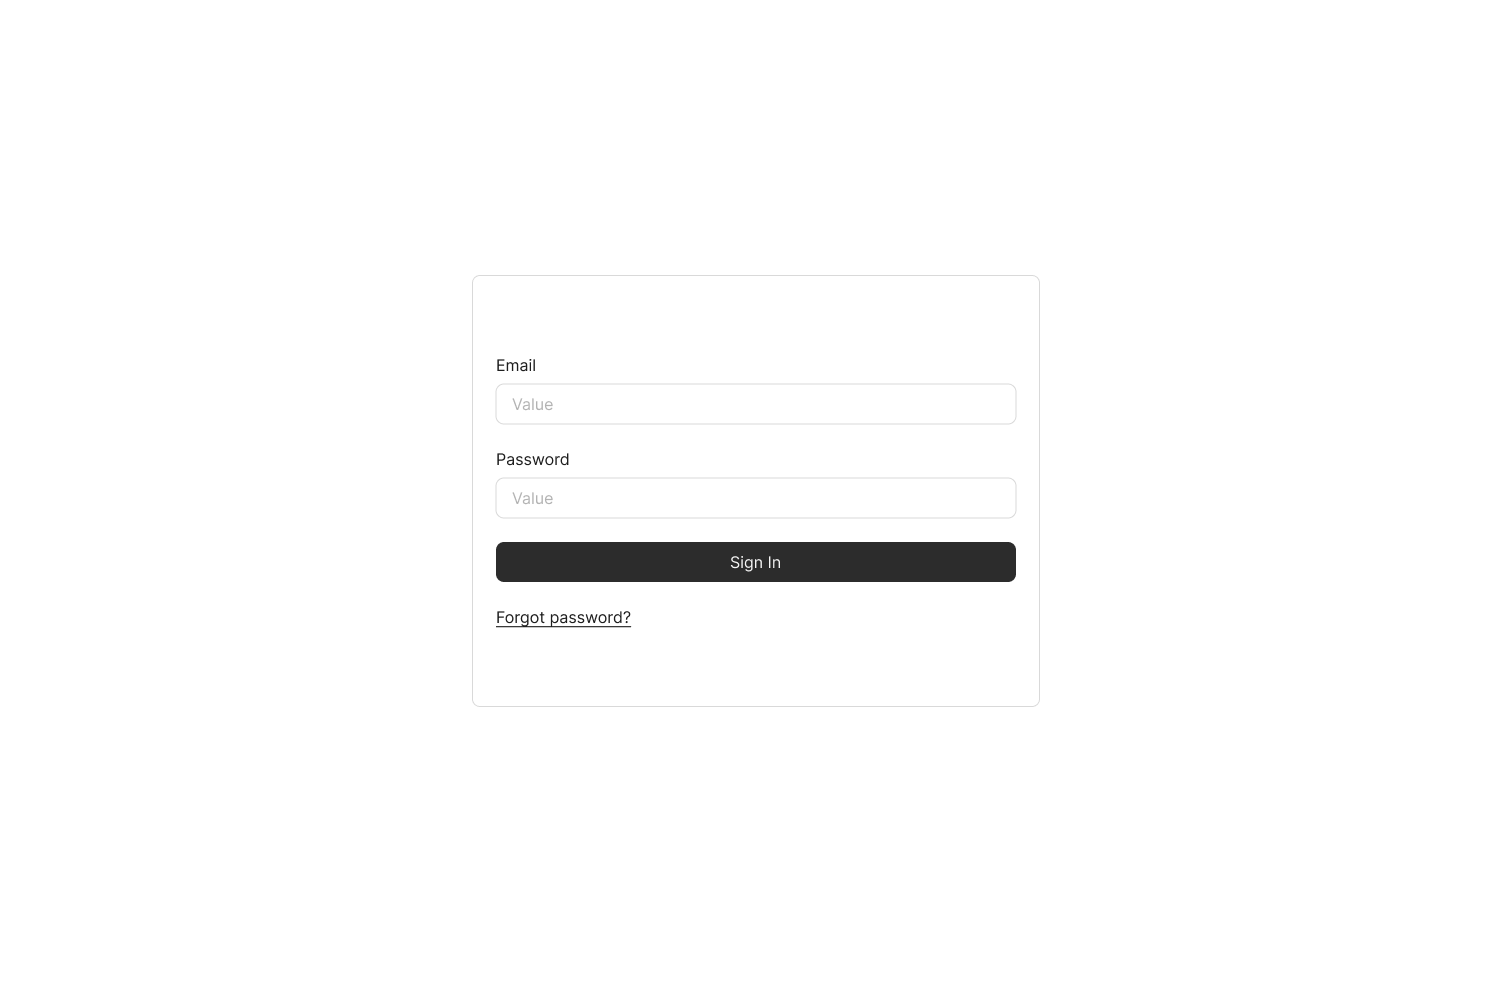
\includegraphics[width=\linewidth]{../../assets/user-interfaces/login.png}
        }
        \subcaption{Log in page}
    \end{minipage}

    \vspace{3em}

    \begin{minipage}{0.45\textwidth}
        \centering
        \fcolorbox{gray}{white}{
            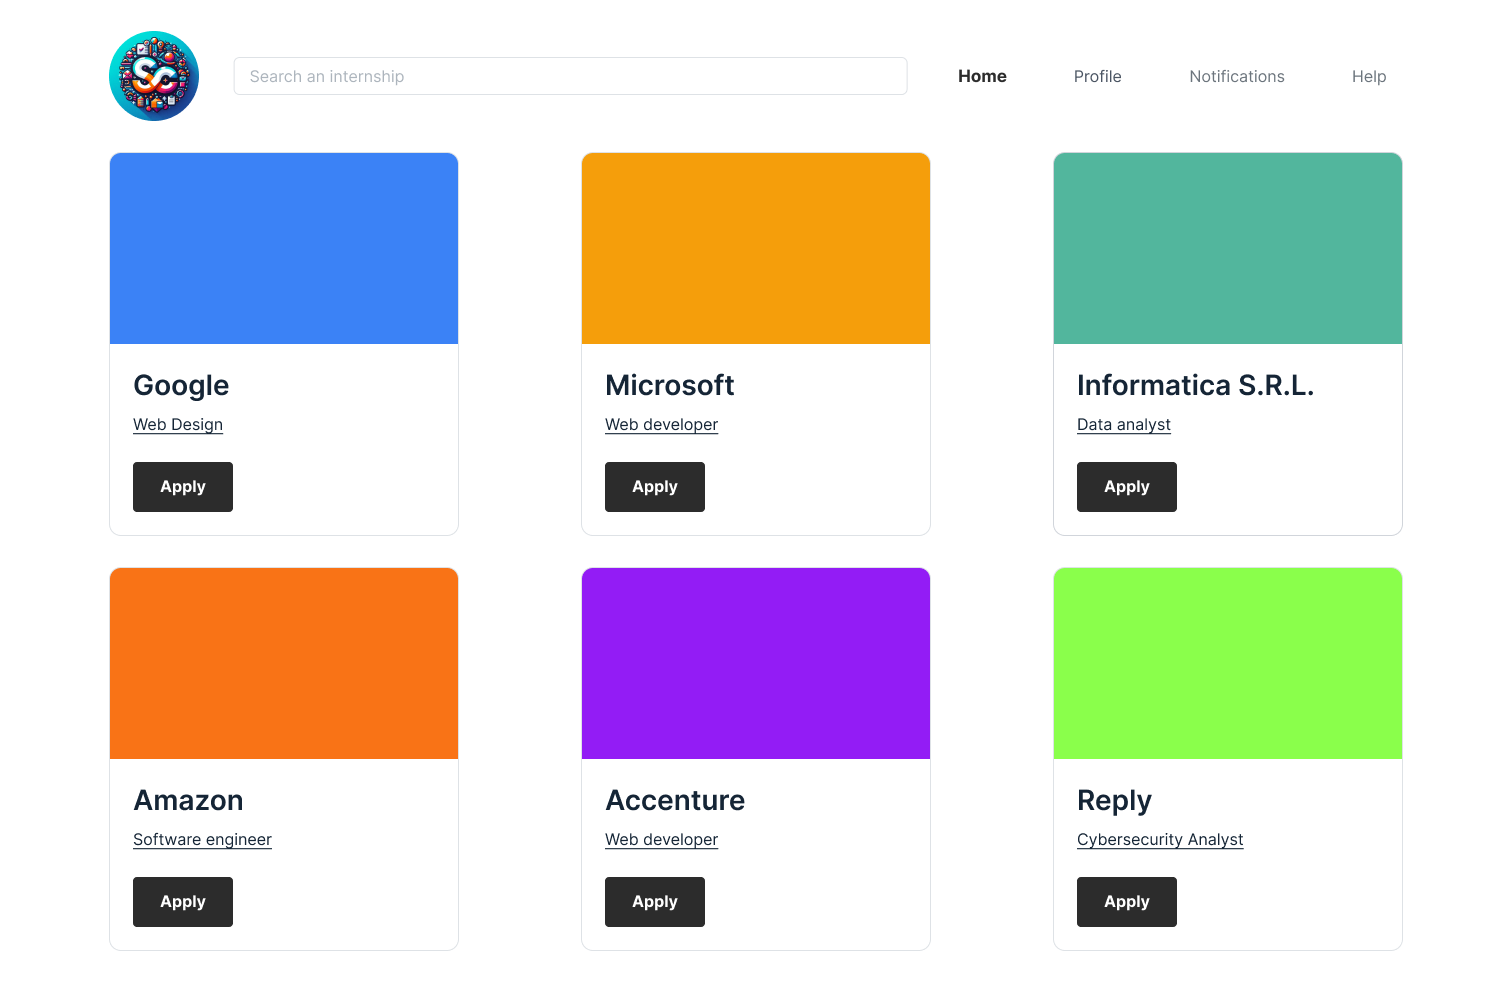
\includegraphics[width=\linewidth]{../../assets/user-interfaces/home.png}
        }
        \subcaption{Home page}
    \end{minipage}
    \hfill
    \begin{minipage}{0.45\textwidth}
        \centering
        \fcolorbox{gray}{white}{
            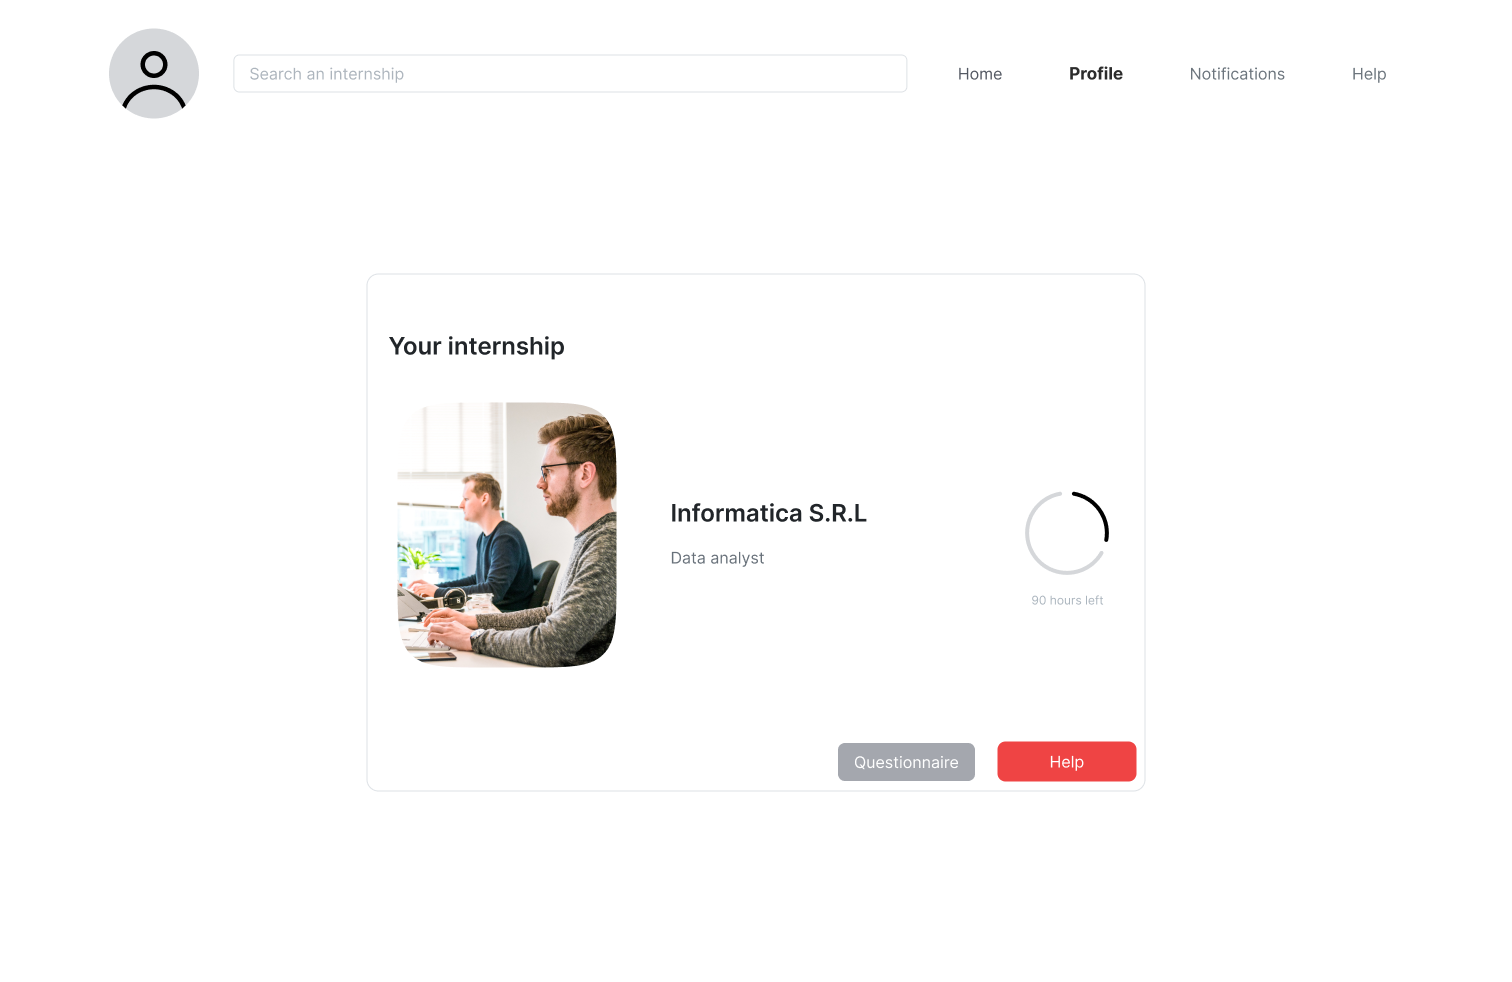
\includegraphics[width=\linewidth]{../../assets/user-interfaces/profile.png}
        }
        \subcaption{Profile page}
    \end{minipage}

    \vspace{3em}

    \begin{minipage}{0.45\textwidth}
        \centering
        \fcolorbox{gray}{white}{
            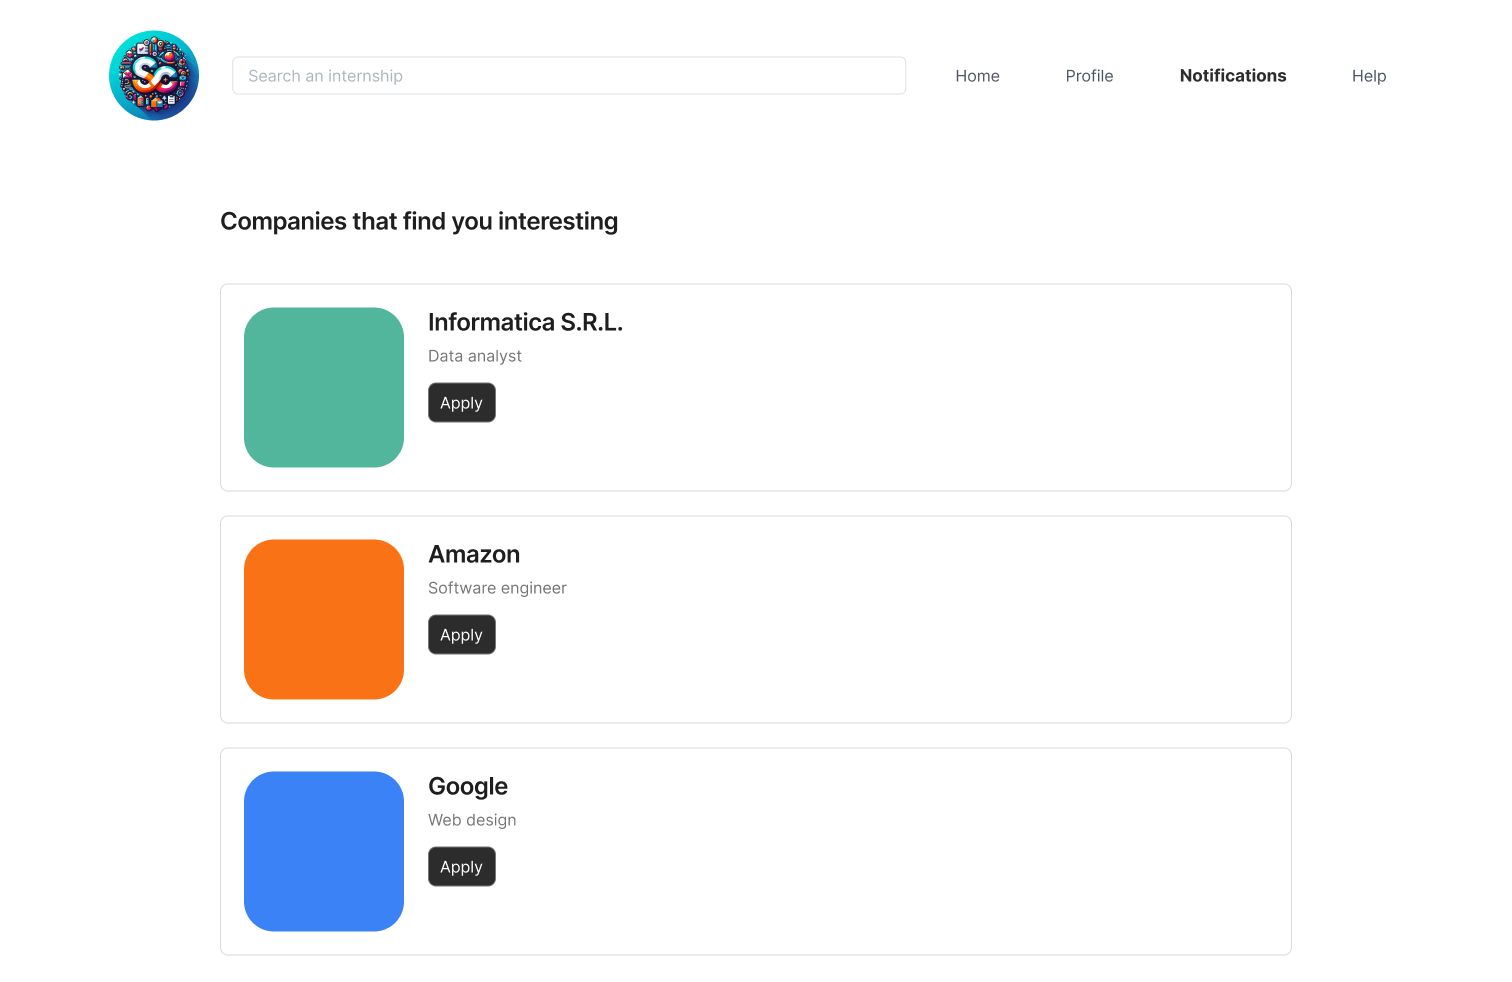
\includegraphics[width=\linewidth]{../../assets/user-interfaces/notifications.png}
        }
        \subcaption{Notifications page}
    \end{minipage}
    \hfill
    \begin{minipage}{0.45\textwidth}
        \centering
        \fcolorbox{gray}{white}{
            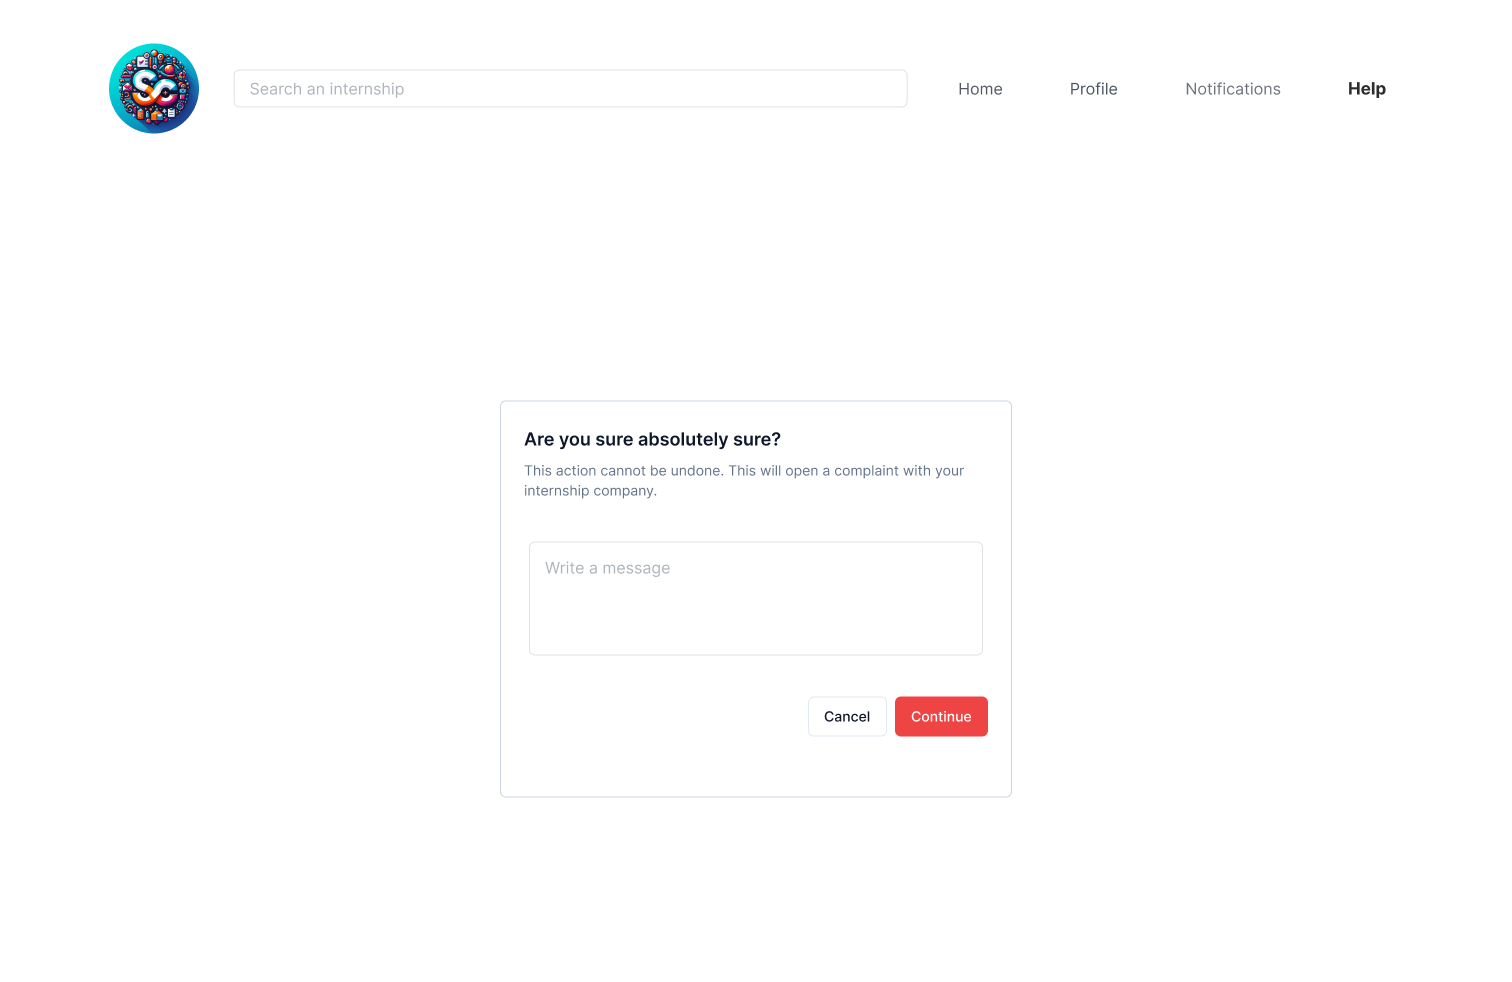
\includegraphics[width=\linewidth]{../../assets/user-interfaces/complaint.png}
        }
        \subcaption{Complaint page}
    \end{minipage}
\end{figure}

\subsection{Hardware Interfaces}

In order be accessed, the platform requires a suitable device with a web browser.

\subsection{Software Interfaces}

The system should integrate a notication service to keep users up of any event on the platform.
An email service is used for the registration process.

\subsection{Communication Interfaces}

The system requires a stable internet connection to work properly.
The connection is used to exchange data between users and the web server, which queries the requested information in a DB.

\section{Functional requirements}

\subsection{Use cases diagram}

\begin{figure}[H]
    \centering
    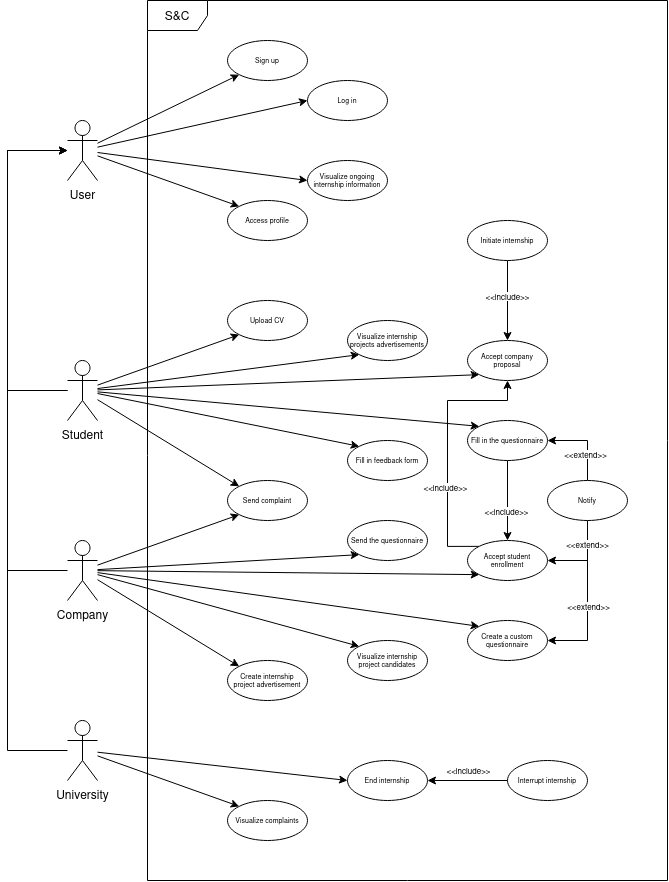
\includegraphics[width=0.75\textwidth]{../../assets/use-cases-diagram.png}
\end{figure}

\subsection{Use cases descriptions}

\begin{enumerate}[label=\textbf{UC\arabic* -}]

\item \subsubsection{StudentSignsUp}

\begin{table}[H]
    \centering
    \begin{tabular}{|l|m{10cm}|}
        \hline \multicolumn{2}{|c|}{\textbf{StudentSignsUp}} \\
        \hline \textbf{Actor} & Student, Students\&Companies, EmailService \\
        \hline \textbf{Entry condition} & The student is not already registered \\
        \hline \textbf{Event flow} &
            \begin{enumerate}[label=\arabic*]
                \item The student opens the sign up page
                \item The student fills in the required informations and clicks the sign up button
                \item The platform checks that the information provided is valid
                \item The platform sends an email through the email service to verify the student account
                \item The student verifies the account via the link found in the email
                \item The platform registers the new student account
                \item The platform shows the student feed page
            \end{enumerate} \\
        \hline \textbf{Exit condition} & The student is registered \\
        \hline \textbf{Exceptions} & The student is already registered (3) \\
        \hline
    \end{tabular}
\end{table}

\begin{figure}[H]
    \centering
    \fcolorbox{black}{white}{
        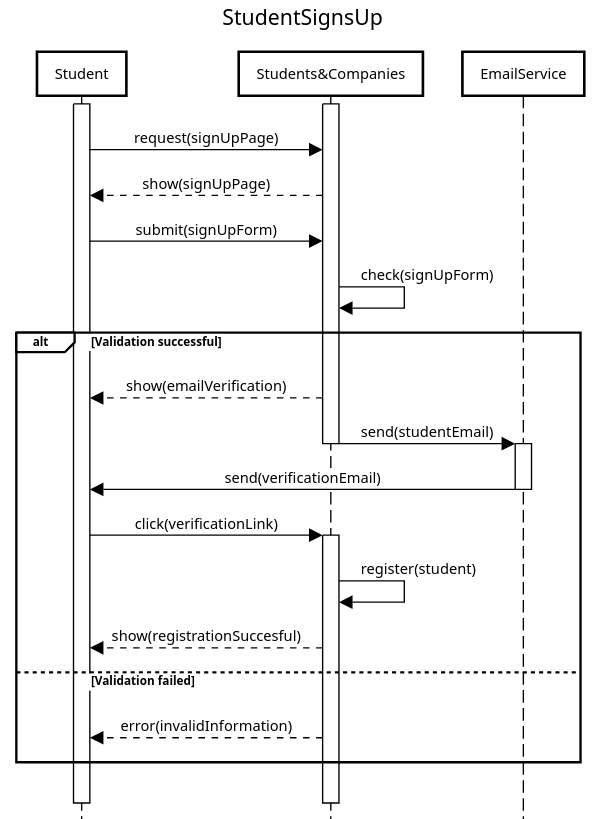
\includegraphics[width=0.75\textwidth]{../../assets/sequence-diagrams/StudentSignsUp.png}
    }
\end{figure}

\item \subsubsection{CompanySignsUp}

\item \subsubsection{UserLogsIn}

\begin{table}[H]
    \centering
    \begin{tabular}{|l|m{10cm}|}
        \hline \multicolumn{2}{|c|}{\textbf{UserLogsIn}} \\
        \hline \textbf{Actor} & Student, Company, University, Students\&Companies \\
        \hline \textbf{Entry condition} & User is registered \\
        \hline \textbf{Event flow} &
            \begin{enumerate}
                \item The user opens the log in page
                \item The platform shows the log in page
                \item The user enters its credentials and clicks the log in button
                \item The platform checks that the account exists and the credentials are correct
                \item The platform shows the home page
            \end{enumerate} \\
        \hline \textbf{Exit condition} & The user is logged in \\
        \hline \textbf{Exceptions} & The student is not registered (4) \\
        \hline
    \end{tabular}
\end{table}

\begin{figure}[H]
    \centering
    \fcolorbox{black}{white}{
        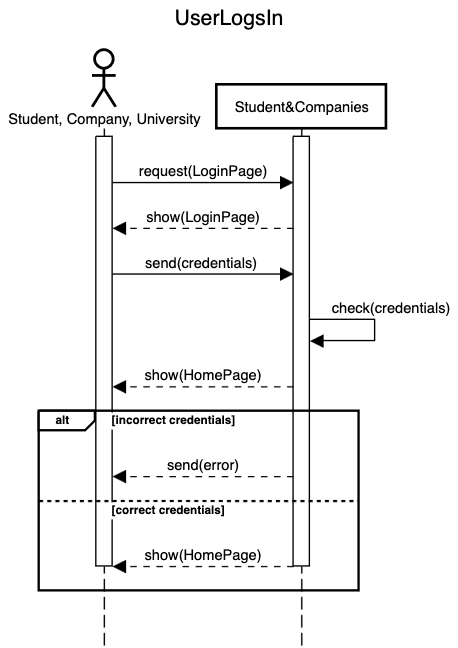
\includegraphics[width=0.5\textwidth]{../../assets/sequence-diagrams/UserLogsIn.png}
    }
\end{figure}

\item \subsubsection{StudentUploadsCV}

\begin{table}[H]
    \centering
    \begin{tabular}{|l|m{10cm}|}
        \hline \multicolumn{2}{|c|}{\textbf{StudentUploadsCV}} \\
        \hline \textbf{Actor} & Student, Students\&Companies \\
        \hline \textbf{Entry condition} & The student is registered \\
        \hline \textbf{Event flow} &
            \begin{enumerate}[label=\arabic*]
                \item The student opens the profile page
                \item The student clicks the upload CV button
                \item The student chooses the CV file and lets it upload
                \item The platform receives the file and stores it
                \item The platform shows the student profile page
            \end{enumerate} \\
        \hline \textbf{Exit condition} & The student profile page shows the new CV \\
        \hline \textbf{Exceptions} & None \\
        \hline
    \end{tabular}
\end{table}

\begin{figure}[H]
    \centering
    \fcolorbox{black}{white}{
        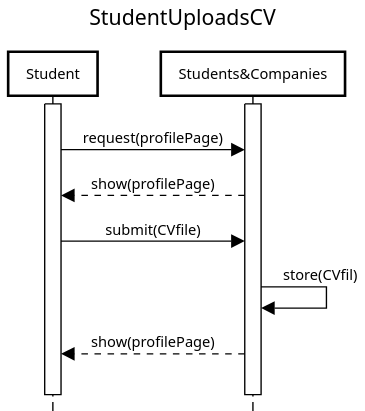
\includegraphics[width=0.45\textwidth]{../../assets/sequence-diagrams/StudentUploadsCV.png}
    }
\end{figure}

\item \subsubsection{CompanyCreatesAdvertisement}

\item \subsubsection{StudentVisualizesAdvertisements}

\begin{table}[H]
    \centering
    \begin{tabular}{|l|m{10cm}|}
        \hline \multicolumn{2}{|c|}{\textbf{StudentVisualizesAdvertisements}} \\
        \hline \textbf{Actor} & Student, Students\&Companies \\
        \hline \textbf{Entry condition} & User is logged in \\
        \hline \textbf{Event flow} &
            \begin{enumerate}
                \item The user opens the home page
                \item The platform finds the advertisements that match the student profile
                \item The platform shows the home page with the advertisements
            \end{enumerate} \\
        \hline \textbf{Exit condition} & The user click on a advertisement or changhe the page \\
        \hline \textbf{Exceptions} & None \\
        \hline
    \end{tabular}
\end{table}

\begin{figure}[H]
    \centering
    \fcolorbox{black}{white}{
        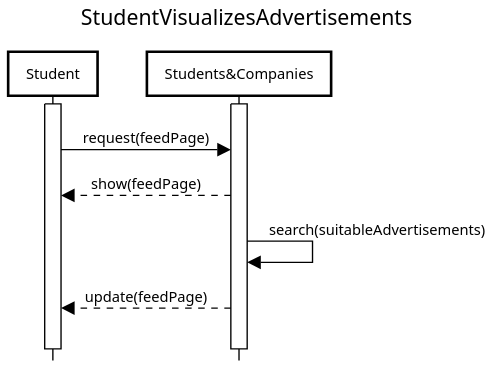
\includegraphics[width=0.5\textwidth]{../../assets/sequence-diagrams/StudentVisualizesAdvertisements.png}
    }
\end{figure}

\item \subsubsection{CompanyVisualizesCandidates}

\begin{table}[H]
    \centering
    \begin{tabular}{|l|m{10cm}|}
        \hline \multicolumn{2}{|c|}{\textbf{CompanyVisualizesCandidates}} \\
        \hline \textbf{Actor} & Company, Students\&Companies \\
        \hline \textbf{Entry condition} & The company is registered \\
        \hline \textbf{Event flow} &
            \begin{enumerate}[label=\arabic*]
                \item The company opens the feed page
                \item The platform searches suitable students to show
                \item The platform sends the potential students list to the company
                \item The company feed page shows the received list
            \end{enumerate} \\
        \hline \textbf{Exit condition} & The company visualizes potential students in the feed \\
        \hline \textbf{Exceptions} & None \\
        \hline
    \end{tabular}
\end{table}

\begin{figure}[H]
    \centering
    \fcolorbox{black}{white}{
        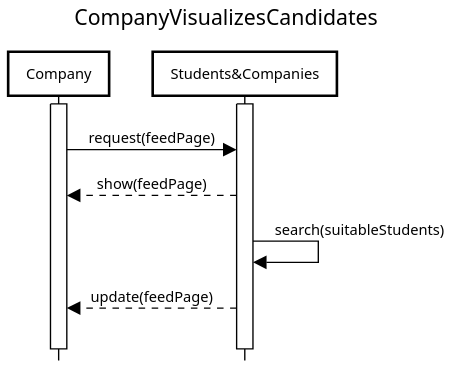
\includegraphics[width=0.55\textwidth]{../../assets/sequence-diagrams/CompanyVisualizesCandidates.png}
    }
\end{figure}

\item \subsubsection{CompanyCreatesQuestionnaire}

\item \subsubsection{StudentFillsQuestionnaire}

\begin{table}[H]
    \centering
    \begin{tabular}{|l|m{10cm}|}
        \hline \multicolumn{2}{|c|}{\textbf{StudentFillsQuestionnaire}} \\
        \hline \textbf{Actor} & Student, Company, Students\&Companies \\
        \hline \textbf{Entry condition} & User is logged in \\
        \hline \textbf{Event flow} &
            \begin{enumerate}
                \item The company creates a questionnaire
                \item The student opens the profile page
                \item The student fills the form in the profile page and clicks the submit button
            \end{enumerate} \\
        \hline \textbf{Exit condition} & The questionnaire button is no longer available \\
        \hline \textbf{Exceptions} & None \\
        \hline
    \end{tabular}
\end{table}

\begin{figure}[H]
    \centering
    \fcolorbox{black}{white}{
        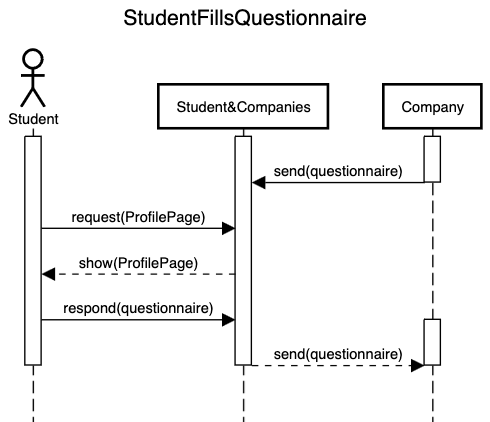
\includegraphics[width=0.5\textwidth]{../../assets/sequence-diagrams/StudentFillsQuestionnaire.png}
    }
\end{figure}

\item \subsubsection{CompanyAcceptsStudentEnrollment}

\begin{table}[H]
    \centering
    \begin{tabular}{|l|m{10cm}|}
        \hline \multicolumn{2}{|c|}{\textbf{CompanyAcceptsStudentEnrollment}} \\
        \hline \textbf{Actor} & Student, Company, Students\&Companies \\
        \hline \textbf{Entry condition} & The student has sent the questionnaire back to the company \\
        \hline \textbf{Event flow} &
            \begin{enumerate}[label=\arabic*]
                \item The company opens the page with the student questionnaire
                \item The company reviews the questionnaire and clicks the accept student button
                \item The platform notifies the student that it has been accepted
                \item The student opens the notifications page and clicks the accept button
                \item The platform checks that all information is valid
                \item The platform initiates the internship between student and company
                \item The platform shows the internship page to the student
                \item The platform notifies the company that the internship has started
            \end{enumerate} \\
        \hline \textbf{Exit condition} & An internship is started between student and company \\
        \hline \textbf{Exceptions} & The student meanwhile accepted another internship (5) \\
        \hline
    \end{tabular}
\end{table}

\begin{figure}[H]
    \centering
    \fcolorbox{black}{white}{
        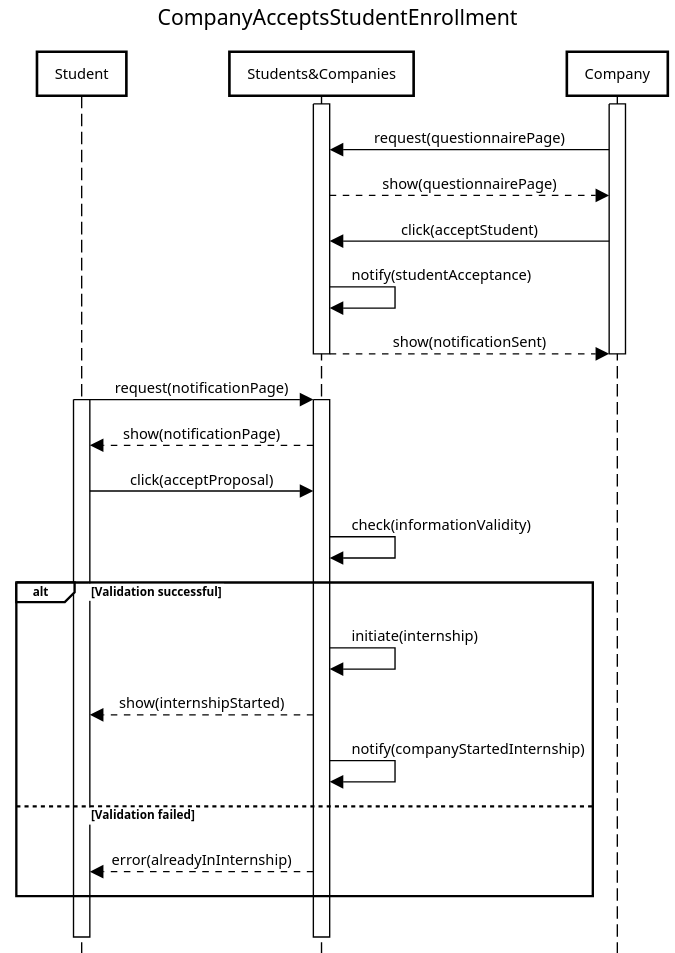
\includegraphics[width=0.8\textwidth]{../../assets/sequence-diagrams/CompanyAcceptsStudentEnrollment.png}
    }
\end{figure}

\item \subsubsection{StudentVisualizesInternshipInformation}

\begin{table}[H]
    \centering
    \begin{tabular}{|l|m{10cm}|}
        \hline \multicolumn{2}{|c|}{\textbf{CompanyVisualizesInternshipsInformation}} \\
        \hline \textbf{Actor} & Company, Students\&Companies \\
        \hline \textbf{Entry condition} & Company is logged in \\
        \hline \textbf{Event flow} &
            \begin{enumerate}
                \item The company opens the profile page
                \item The company selects an internship from the list of all interships
                \item The system shows the internship information and the student enrolled
            \end{enumerate} \\
        \hline \textbf{Exit condition} & The company displays all the information \\
        \hline \textbf{Exceptions} & None \\
        \hline
    \end{tabular}
\end{table}

\begin{figure}[H]
    \centering
    \fcolorbox{black}{white}{
        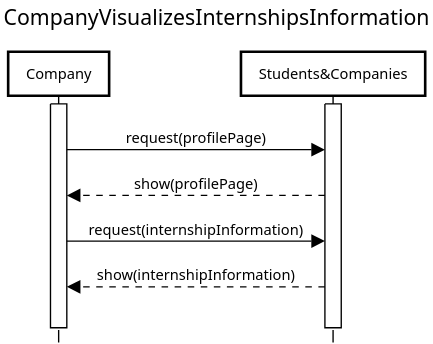
\includegraphics[width=0.5\textwidth]{../../assets/sequence-diagrams/CompanyVisualizesInternshipsInformation.png}
    }
\end{figure}


\item \subsubsection{CompanyVisualizesInternshipsInformation}

\item \subsubsection{StudentSendsComplaint}

\begin{table}[H]
    \centering
    \begin{tabular}{|l|m{10cm}|}
        \hline \multicolumn{2}{|c|}{\textbf{StudentSendsComplaint}} \\
        \hline \textbf{Actor} & Student, University, Students\&Companies \\
        \hline \textbf{Entry condition} & The student is currently enrolled in an internship \\
        \hline \textbf{Event flow} &
            \begin{enumerate}[label=\arabic*]
                \item The student opens the complaints page
                \item The student fills in the complaint text box and clicks the send button
                \item The platform notifies the university of the complaint
                \item The university opens the notifications/complaint page and views the complaint
            \end{enumerate} \\
        \hline \textbf{Exit condition} & The university visualizes the complaint \\
        \hline \textbf{Exceptions} & None \\
        \hline
    \end{tabular}
\end{table}

\begin{figure}[H]
    \centering
    \fcolorbox{black}{white}{
        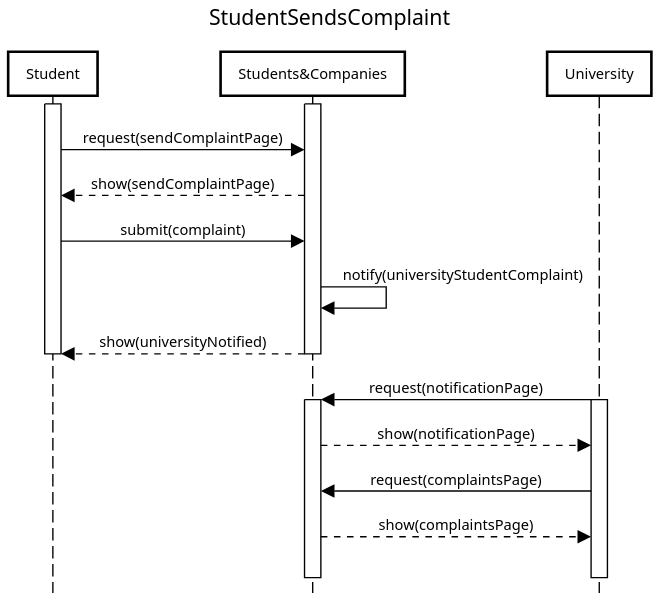
\includegraphics[width=0.75\textwidth]{../../assets/sequence-diagrams/StudentSendsComplaint.png}
    }
\end{figure}

\item \subsubsection{CompanySendsComplaint}

\item \subsubsection{UniversityVisualizesComplaints}

\item \subsubsection{UniversityEndsInternship}

\begin{table}[H]
    \centering
    \begin{tabular}{|l|m{10cm}|}
        \hline \multicolumn{2}{|c|}{\textbf{UniversityEndsInternship}} \\
        \hline \textbf{Actor} & Student, Company, University, Students\&Companies \\
        \hline \textbf{Entry condition} & Student and company are currently linked in an internship \\
        \hline \textbf{Event flow} &
            \begin{enumerate}[label=\arabic*]
                \item The university opens the ongoing internships page and clicks the interruption button
                \item The platform registers the internship as concluded
                \item The company is notified of the internship conclusion
                \item The student is notified of the internship conclusion
            \end{enumerate} \\
        \hline \textbf{Exit condition} & The internship is registered as concluded \\
        \hline \textbf{Exceptions} & None \\
        \hline
    \end{tabular}
\end{table}

\begin{figure}[H]
    \centering
    \fcolorbox{black}{white}{
        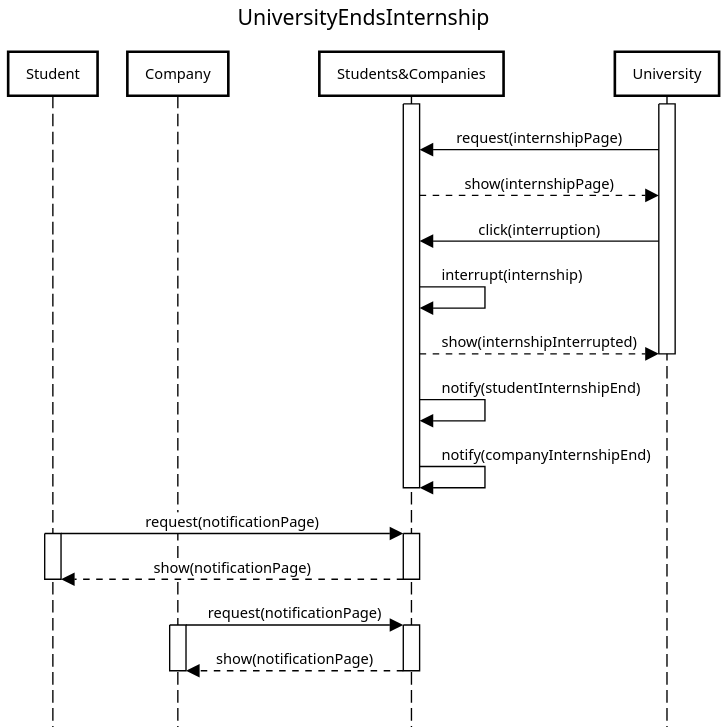
\includegraphics[width=0.75\textwidth]{../../assets/sequence-diagrams/UniversityEndsInternship.png}
    }
\end{figure}

\item \subsubsection{InternshipExpires}

\item \subsubsection{StudentFillsFeedbackForm}

\end{enumerate}

\subsection{Use cases sequence diagrams}

\subsection{Use cases mapping}

\section{Performance requirements}

\subsection{Specific requirements}

\section{Design constraints}
\subsection{Standards compliance}
\subsection{Hardware limitations}
\subsection{Any other constraint}

\section{Software system attributes}
\subsection{Reliability}
\subsection{Availability}
\subsection{Security}
\subsection{Maintainability}
\subsection{Portability}